\vspace{-2in}
\chapter{Work Done}
The algorithms that have been considered for the project are stated below :
\begin{itemize}
\item Biased Random Sampling
\item Honey Bee Foraging
\item Hybrid Algorithm
\end{itemize}

\section{Theory}
\subsection{Biased Random Sampling}
In this type of approach we need to construct a network comprising of virtual nodes 
which represent all the resources present on the server to represent the total load.
The indegree of the node corresponds to the free resources of the server such that \cite{Madhu}:

\begin{itemize}
\item Whenever a node executes a job, it deletes an incoming edge, which indicates reduction
in the availability of free resources.
\item After completion of a job, node creates an incoming edge which indicates an increase
in availability of the resources.
\end{itemize} 
The working of the algorithm can be understood by the following pseudo code :
%\begin{algorithmic}
%\STATE $b \gets log(n)$ \COMMENT{n\hspace*{1mm}-\hspace*{1mm}Network\hspace*{1mm}Size}
%\FOR{Node\hspace*{1mm}that\hspace*{1mm}Receives\hspace*{1mm}a\hspace*{1mm}New\hspace*{1mm}Process}
%\STATE $/^*Create\hspace*{1mm}and\hspace*{1mm}send\hspace*{1mm}token\hspace*{1mm}to\hspace*{1mm}randomly\hspace*{1mm}selected\hspace*{1mm}neighbour^*/$
%\STATE $Job.walklength \gets 1$
%\STATE $/^*Select\hspace*{1mm}a\hspace*{1mm}neighbour\hspace*{1mm}using\hspace*{1mm}probability\hspace*{1mm}based\hspace*{1mm}function^*/$
%\STATE $Randomselect(node)$
%\STATE $/^*Send\hspace*{1mm}job\hspace*{1mm}to\hspace*{1mm}selected\hspace*{1mm}neighbour^*/$
%\STATE $Send(job,neighbour)$
%\ENDFOR
%\end{algorithmic}

\begin{verbatim}
b = log n  //n - network size

For any node that recieves a new process 
    /*Create and send token to 
    randomly selected neighbour*/
    job.walklength = 1
    /*Select a neighbour using 
    probability based function*/
    Randomselect(node)
    /*Send job to selected neighbour*/
    Send(job,neighbour)

For any node that recieves token
    /*Update token if needed and send it 
    to neighbour selected by the function*/
    if job.walklength < b then
        neighbour = Randomselect(node)
        Send(job,neighbour)
    else
    /*Execution of job on node 
    indiacted by the token*/
        Execute(job)
    endif
\end{verbatim}

\subsection{Honeybee Foraging}
The first job, on being sent into the network
of servers acts as a scout providing information
on the availability of resources at each server.
This information is published on an advert board
which is referenced by the incoming jobs. Based
on the fitness function, jobs attach themselves
to the server and simultaneously update the advert
board.\\[0.2cm]
The working of the algorithm can be understood by the following pseudo code :
\begin{verbatim}
/*Scout on entering network*/
TraverseNetwork(scout)
CreateAdvertBoard()

For all incoming jobs
    /*Checking for the best server*/
    node = fitness(job)
    /*Job Execution*/
    Attach(node,job)
    /*Updating advert board with 
     current status of resources*/
    UpdateAdvertBoard(node,job) 
\end{verbatim}

\subsection{Proposed Hybrid Algorithm}
This algorithm is a combination of biased random sampling and honeybee
foraging. The incoming jobs are scheduled on the basis of their job size.\\[0.2cm]
It has been experimentally observed while working on the above two algorithms that the biased random sampling gives a more consistent result
during the execution of jobs of size one.\\[0.2cm]
The working of the algorithm can be understood by the following pseudo code :
\begin{verbatim}
/*Jobs on entering network*/
if jobsize==1 then
    BiasedRandomSampling(job);
else
    HoneyBeeForaging(job);
endif
\end{verbatim}
 
\section{Implementation}
An array of 100 jobs with random jobsize and execution time
and an adjacency matrix of a fixed network of servers are given
as inputs.The server network being created by the adjacency matrix forms a directed graph which
allows for easy traversal between the servers.
\begin{itemize}
\item \textbf{Nodequeue:} This is a list of all the jobs being executed by the particular server including the job size, execution time and the time at which
the job was allocated to the server.
\item \textbf{NodeArrayList:} The list of all the servers in the network and their
accompanying node queue are contained here.
\end{itemize}
The increaseindegree(), common to all the algorithms, traverses 
the array list associated with each job and checks if any job 
that was being executed by each server has been completed. 
This is done by comparing the current time with the sum of 
the execution time required for the job and the time at which it 
was allocated to the server. On completion of the jobs, the array list is updated accordingly and the resources available with the server are incremented.\\[0.2cm]
The timer functions are as follows: jobs are sent every one 
second and if the job cannot be allocated presently to any 
server due to lack of resources then it waits for two seconds before trying again.

\subsection{Biased Random Sampling}
\begin{itemize}
\item \textbf{BiasedRandomWalk:} The selectwalk() initially checks for the availability of the resources with the help of increaseindegree() and uses the hopcount which gives the length of the walk. It randomly chooses a server and checks if the job can be allocated to be followed by the invocation of selectneighbour(). If no resources are available, then it randomly chooses another server and continues the above process. The selectneighbour() probabilistically chooses the next best server based on the resources available in each of the neighbor. This neighbor selection is done till the hopcount value is reached. The send() compares the resources between the last two servers and updates the token with the better value. It then updates the resource information of the server to which the job has been allocated and finally returns the server node.
\item \textbf{GraphBiased:} The creategraph() contains the server network (represented by an adjacency matrix) and also the information pertaining to the availability of resources with each server. An object of the BiasedRandomWalk class is created and we check for the availability of resources in the network. If resources are unavailable, then the next job to be allocated waits. Only when resources are made available the process of random selection starts.
\end{itemize}

\subsection{Honeybee Foraging}
\begin{itemize}
\item \textbf{Fitness:} The class contains select() which initially calls increaseindegree() to update the current resource status of the servers. A traversal of the server network is done whereby for each server we calculate the difference in the resources currently available and the resources requested. The job is then allocated to the server for which the difference is small. The resource available for that server is decremented accordingly and it finally returns the best fit server.
\item \textbf{GraphHoneyBee:} The server network is represented with an adjacency matrix. The creategraph() forms the network and calculates the available resources with each server. This is called when the scout job is sent. The fitness() is invoked which does the job allocation. If job could not be allocated because of lack of resources, then the current job waits and calls the increaseindegree() to get updated resource information.
\end{itemize}

\subsection{Proposed Hybrid Algorithm}
This algorithm makes use of the BiasedRandomWalk and Fitness classes from the above two algorithms. 
\begin{itemize}
\item \textbf{Hybrid:} The creategraph() contains the server network (represented by the adjacency matrix)  and also about the resources available with each server. Objects of BiasedRandomWalk and Fitness classes are created. The job() receives each job and then checks if any resources are available in the network and then calls the selectjob() (after waiting, if resources were unavailable). If the job requires only one resource, then the biased random sampling algorithm is used while the honeybee foraging algorithm is used otherwise. The selectjob() chooses the algorithm for each particular job and then sends the job to the respective functions in BiasedRandomWalk or Fitness. 
\end{itemize}
The set of 100 jobs is executed by the algorithm and its total execution time is recorded. This process is repeated for 100 times and an average execution time is obtained for each algorithm.

\section{Analysis}
\subsection{Biased Random Sampling}
In the biased random sampling algorithm, for every batch of hundred jobs, small changes in the range of seconds were obtained. The change which occurred is because of the delay being caused due to unavailability of resources. A random node is selected only initially and the walk is taken based on the probabilistic function and hence the walk only goes up to the value of hopcount (which is the same) for every allocation of job. The time taken for load balancing of every job varies by seconds because the algorithm looks for a server with maximum resources available and then tries to allocate the job. So, overheads are obtained because of finding the path for every job followed by comparing it; even though only finally the job size is checked.
\begin{center}
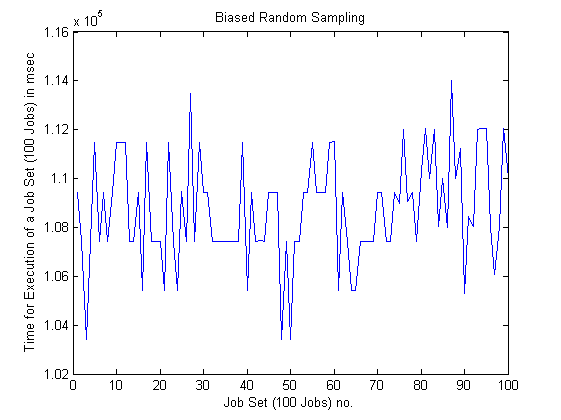
\includegraphics[width=0.9\textwidth]{biased}\\[0.3cm]
\end{center}

\subsection{Honeybee Foraging}
In the honey bee foraging algorithm, the running time for the batch of jobs is almost same only varying by milliseconds. This change is due to the delay caused by the unavailability of resources since the other jobs are utilizing all the servers in the network. The portions of consistent timing are due to the traversal of the same advert board by every job being sent into the network. Since the advert board is a graph traversal with a list of jobs attached with each node, the algorithm takes almost similar time for the traversal in each case since the job size does not vary drastically.
\begin{center}
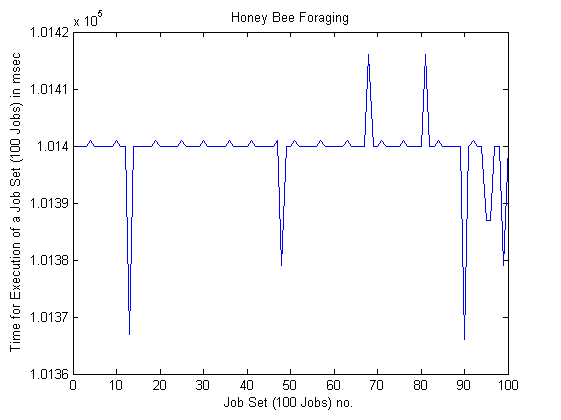
\includegraphics[width=0.9\textwidth]{honeybee}\\[0.3cm]
\end{center}

\subsection{Proposed Hybrid Algorithm}
In the proposed hybrid algorithm, the timing pattern shows a divergence in the range of seconds with almost no perfectly same running time in a batch of ten. This variation is due to the unavailability of resources which causes a delay. This is because of the server being chosen, for a particular job, by both the algorithms. While biased chooses the server with the maximum number of resources, honey bee goes in for a more optimal selection taking a best fit approach.
\begin{center}
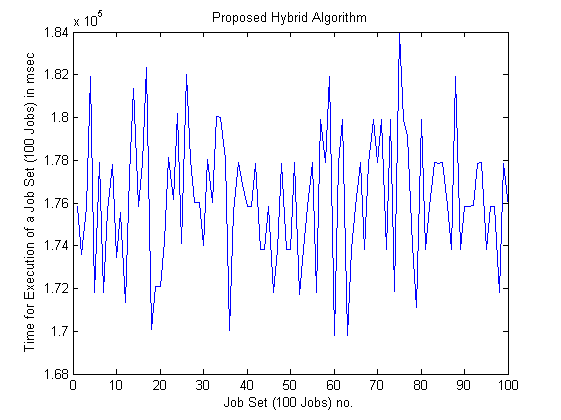
\includegraphics[width=0.9\textwidth]{hybrid}\\[0.3cm]
\end{center}
The hybrid algorithm uses the biased random sampling only for a probability of 1/5 (job size has been bound to a maximum of 5) to get a better consistent timing pattern as has been experimentally observed below; whereas the honeybee algorithm is selected with a probability of 4/5. If we consider a case where a biasing function has been applied such that the probability of choosing either of the algorithm is same, then a more inconsistent graph with larger number of peaks and dips are obtained because of the above explained contradiction.
\begin{center}
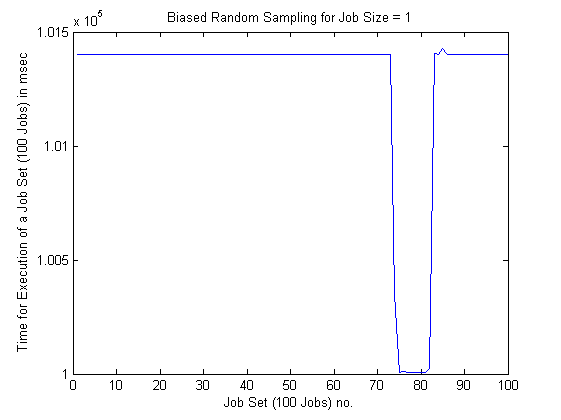
\includegraphics[width=0.9\textwidth]{biased1}\\[0.3cm]
\end{center}
All the three algorithms show changes only in the range of milliseconds to seconds for a batch of hundred jobs being run hundred times. While biased takes 10870 ms, honey bee runs in 10140 ms and hybrid in 17617 ms for a batch of 100 jobs on an average. This clearly shows that the honey bee algorithm is the best approach of all the algorithms considered. Though honey bee has a more consistent run time (the inconsistency occurs due to reaching a state where no resources are available) as compared to biased (the inconsistency being caused by the delays due to the checking of job size only finally), the hybrid algorithm has a highly inconsistent run time graph because of entering the state more due to the contradiction in server selection between the two algorithms.
